% 2D Image with indices
% Author: Peter Steinbach
\documentclass[tikz]{standalone}
%\documentclass[dvisvgm]{standalone}
%\def\pgfsysdriver{pgfsys-tex4ht.def}
\usepackage{tikz}
\usetikzlibrary{calc,trees,positioning,arrows.meta,chains,shapes.geometric,shapes.arrows,%
    decorations.pathreplacing,decorations.pathmorphing,shapes,%
    matrix,shapes.symbols,fit,backgrounds}

 \pgfdeclarelayer{back}
 \pgfsetlayers{background,back,main}


\makeatletter
\makeatother

\begin{document}
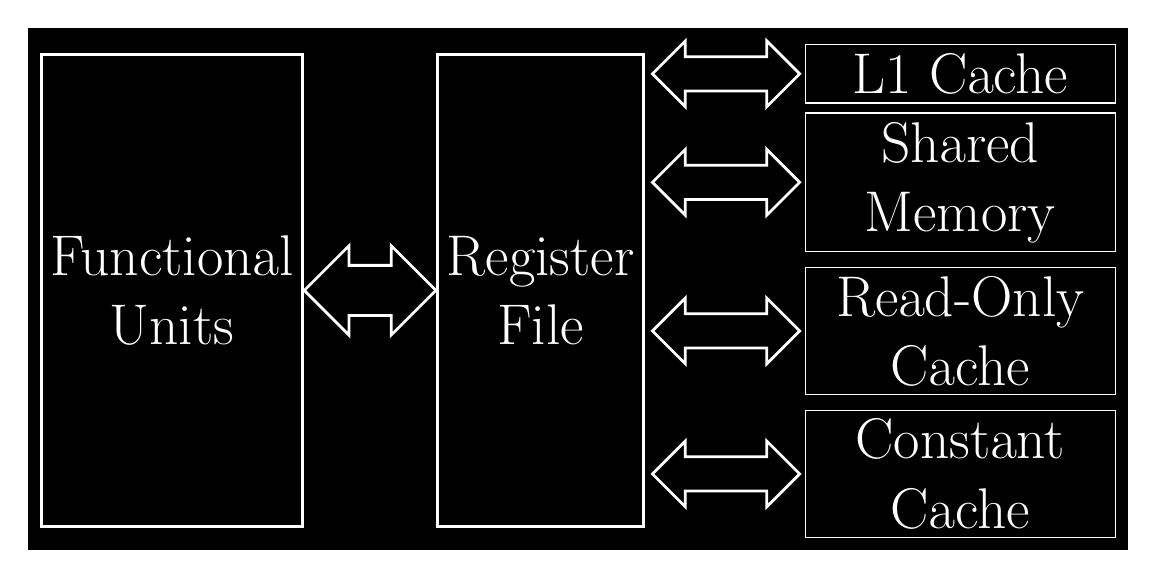
\begin{tikzpicture}[block/.style={
    draw,
%    fill=white,
    rectangle, 
    text width={width("Read-Only Cache")+1cm},
    align=center,
    font=\huge},
  show background rectangle, 
  background rectangle/.style={fill=black},
  color=white,
  help lines/.style={color=lightgray,line width=.2pt},
  ]

  \node (FUs) [very thick,draw,rectangle, minimum width={width("Functional")+.5cm}, minimum height=6cm,font=\huge,align=center] at(0,0) {Functional\\Units};
  
  \node (Regs) [very thick,draw,rectangle, minimum width={width("Register")+.5cm}, minimum height=6cm,font=\huge,align=center] at($(FUs.east)+(3,0)$) {Register\\File};

  \node (ro_regs) at($(Regs.east) + (4,0)$) {};

  \node (L1Cache) [block] at($(ro_regs)+(0,2.75)$) {L1 Cache};
  \node (ShMem) [block] at($(L1Cache.south)+(0,-1)$) {Shared Memory};

  \node (RoCache) [block] at($(ShMem.south)-(0,1)$) {Read-Only Cache};
  \node (ConstCache) [block] at($(RoCache.south)-(0,1)$) {Constant Cache};

  \node [double arrow, draw, line width=1pt,font=\huge,inner xsep=.5cm,inner ysep=.3cm] at($(FUs.east)!.5!(Regs.west)$) {};

  \node [double arrow, draw, line width=1pt,font=\huge,inner xsep=.7cm,inner ysep=.2cm, double arrow head extend=.2cm] at($(L1Cache.west)+(-1,0)$) {};

  \node [double arrow, draw, line width=1pt,font=\huge,inner xsep=.7cm,inner ysep=.2cm, double arrow head extend=.2cm] at($(ShMem.west)+(-1,0)$) {};

  \node [double arrow, draw, line width=1pt,font=\huge,inner xsep=.7cm,inner ysep=.2cm, double arrow head extend=.2cm] at($(RoCache.west)+(-1,0)$) {};

  \node [double arrow, draw, line width=1pt,font=\huge,inner xsep=.7cm,inner ysep=.2cm, double arrow head extend=.2cm] at($(ConstCache.west)+(-1,0)$) {};

\end{tikzpicture}
\end{document}
